\documentclass[11pt]{article}

\usepackage[margin=1in]{geometry}
\usepackage{amsmath,amssymb,amsthm}
\usepackage{graphicx}
\usepackage[hidelinks]{hyperref}
\usepackage{enumitem}

\setlength{\parindent}{0pt}
\setlength{\parskip}{0.6em}
\setlist[itemize]{leftmargin=1.5em}

\newtheorem{theorem}{Theorem}
\newtheorem{lemma}{Lemma}

\newcommand{\R}{\mathbb{R}}
\newcommand{\cL}{\mathcal{L}}
\newcommand{\Pos}{\mathcal{P}}
\newcommand{\Mom}{\mathcal{M}}
\newcommand{\ev}{\operatorname{ev}}
\newcommand{\Pic}{\operatorname{Pic}}
\newcommand{\car}{\mathcal{C}}

\begin{document}

\begin{center}
{\Large Full Solution Packet}\\[0.3em]
{\large Multiple real points at infinity force non-flat moments}\\[0.45em]
\textbf{Status:} candidate full solution, likely valid\\
\textbf{Target:} the conjecture after Example 7.2.3 of arXiv:2407.06017
\end{center}

\section*{Source and exact conjecture}

The source is Baldi--Blekherman--Sinn,
\emph{Nonnegative Polynomials and Moment Problems on Algebraic Curves}
\cite{BBS}. Under its standing assumptions, the projective closure
$\overline X\subset\mathbb P^2$ is a smooth totally real plane cubic and
$X=\overline X\setminus S$ is an affine part, where
$S=\overline X(\R)\setminus X(\R)$ is the finite set of real points at
infinity.

\begin{center}
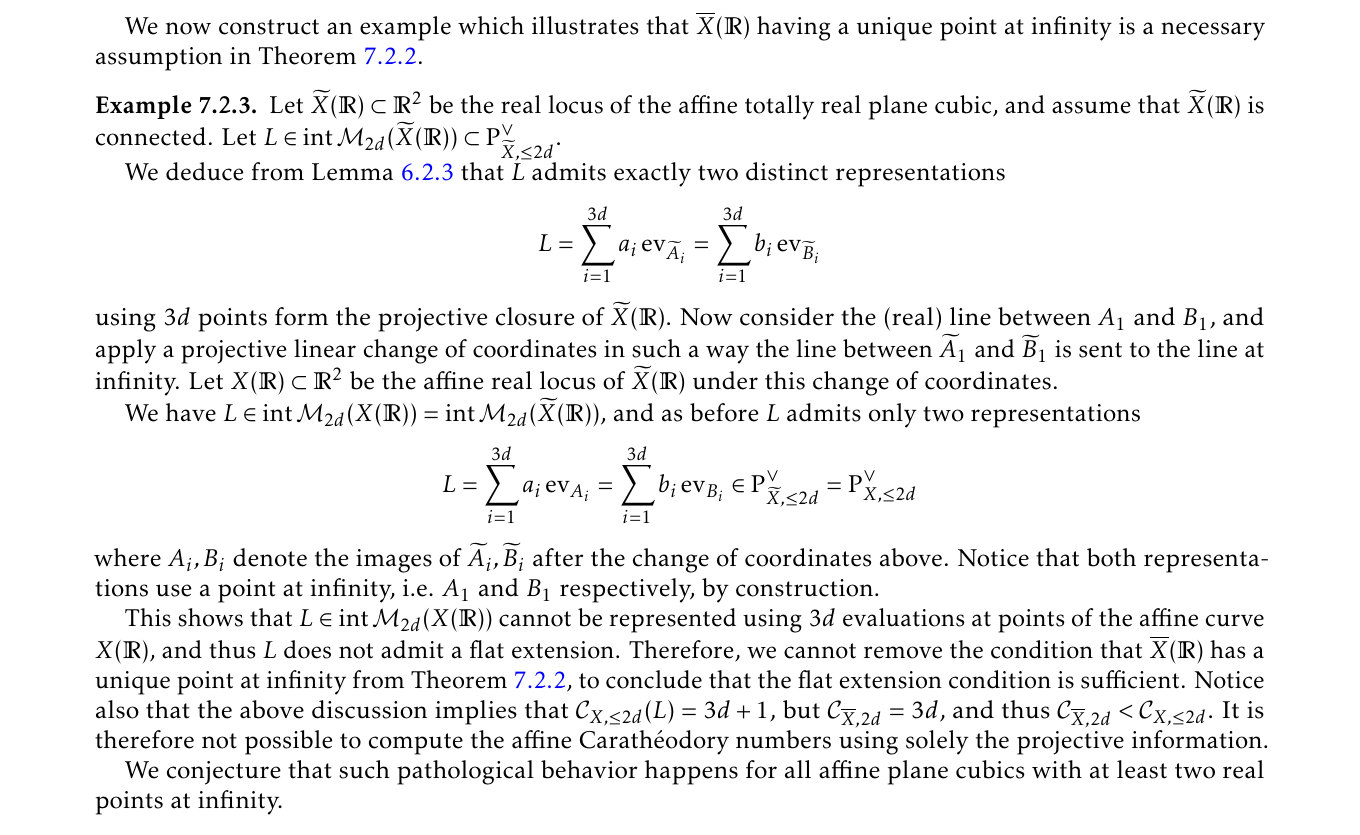
\includegraphics[width=\textwidth]{figures/open_conjecture_crop.png}
\end{center}

For degree $2d$, put $r=3d$. The source constructs one connected example
with a moment functional whose projective Carath\'eodory number is $r$ but
whose affine Carath\'eodory number is $r+1$, and conjectures that this
pathology occurs for every affine plane cubic with at least two real points
at infinity. Equivalently, ordinary positive flat extension is not sufficient
in all such cases.

\section*{Result}

\begin{theorem}\label{thm:main}
Let $\overline X\subset\mathbb P^2$ be a smooth totally real plane cubic,
let $X=\overline X\setminus S$, and suppose that $S$ contains at least two
distinct real points. For every integer $d\geq1$, there exists
\[
 L\in\Mom_{2d}(X(\R))
\]
which has no positive flat extension from degree $2d$ to degree $2d+2$.

If $\overline X(\R)$ is connected, $L$ may be chosen so that
\[
 \car_{\overline X,2d}(L)=3d,
 \qquad
 \car_{X,\leq2d}(L)=3d+1.
\]
Together with the disconnected case proved in Theorem 7.2.4 of the source,
this proves the conjecture after Example 7.2.3.
\end{theorem}

\section*{Proof intuition}

Choose two prescribed points $P,Q\in S$. On the circle
$\overline X(\R)$, construct a reduced real divisor
\[
 D=T_1+\cdots+T_{6d}\in|\mathcal O_{\overline X}(2d)|
\]
which contains $P,Q$ in positions of opposite parity. If $q$ is a real
section with divisor $D$, the residue theorem applied to
$(h/q)\omega$ gives the unique relation among the evaluations at the
$T_i$. Its coefficients alternate in sign around the circle. Hence the
relation splits into two positive $3d$-atomic representations of one
functional $L$, one containing $P$ and the other containing $Q$.

A generic choice of $D$ makes $L$ an interior projective moment functional.
The source's Lemma 6.2.3 then says that these are its only two minimal
projective representations. Thus no $3d$-atomic representation avoids
$S$. On the other hand, the source's Lemma 6.2.6 supplies a
$(3d+1)$-atomic representation avoiding any prescribed finite set, hence
avoiding $S$. This proves the claimed affine/projective rank gap and rules
out a flat extension.

\section*{Two lemmas}

Set
\[
 N=6d,\qquad r=N/2=3d,\qquad
 \cL=\mathcal O_{\overline X}(2d),
\]
and write $H$ for a hyperplane divisor on $\overline X$. Thus
$\cL\cong\mathcal O_{\overline X}(2dH)$,
$\deg\cL=N$, and $\dim H^0(\overline X,\cL)=N$.

\begin{lemma}[A prescribed alternating real divisor]\label{lem:divisor}
Assume that $\overline X(\R)$ is connected. Given distinct
$P,Q\in\overline X(\R)$, there is a reduced totally real divisor
\[
 D=T_1+\cdots+T_N\in|\cL|
\]
containing $P$ and $Q$, such that $P$ and $Q$ have opposite parity in the
cyclic order of the $T_i$. Moreover, if
\[
 A=T_1+T_3+\cdots+T_{N-1},
 \qquad
 B=T_2+T_4+\cdots+T_N,
\]
then the divisor can be chosen so that
\begin{equation}\label{eq:not-torsion}
 2A\not\sim\cL .
\end{equation}
\end{lemma}

\begin{proof}
The connected real elliptic curve $\overline X(\R)$ is a circle group.
Choose a group coordinate
$\theta:\overline X(\R)\to\R/\mathbb Z$. By Abel's theorem, a real divisor
of degree $N$ belongs to $|\cL|$ precisely when the sum of its points has
the fixed value corresponding to $\cL$ in
$\Pic^N(\overline X)(\R)$.

Of the two open arcs between $P$ and $Q$, choose one, denoted $I$, whose
length in the group coordinate is at least $1/2$. Put all the remaining
$m=N-2\geq4$ points in $I$. On the ordered configuration simplex
\[
 a<t_1<\cdots<t_m<b
\]
for a lift $I=(a,b)$, the ordinary sum $t_1+\cdots+t_m$ ranges through
the interval $(ma,mb)$. Its length is
$m(b-a)\geq2$, so its image modulo $\mathbb Z$ is the whole circle.
We can therefore choose distinct points in $I$ so that, together with
$P,Q$, their Abel sum is the class of $\cL$. This gives $D\in|\cL|$.

The number of chosen points on one arc from $P$ to $Q$ is either $0$ or
$m$, and $m$ is even. Thus $P,Q$ have opposite parity in the cyclic
ordering of $D$.

It remains to impose \eqref{eq:not-torsion}. The fixed-sum configuration
has positive dimension. Move one point assigned to $A$ by a small amount
$t$ and an adjacent point assigned to $B$ by $-t$. The Abel sum of $D$
stays fixed while the Abel sum of $A$ varies. The forbidden condition
$2A\sim\cL$ asks that $A-dH$ be one of finitely many $2$-torsion
classes. A generic small variation therefore avoids it while preserving
distinctness and cyclic order.
\end{proof}

\begin{lemma}[Alternating residue circuit]\label{lem:residue}
Let $D=T_1+\cdots+T_N\in|\cL|$ be reduced and totally real, written in
cyclic order. There is a unique relation, up to nonzero scale,
\[
 \sum_{i=1}^{N}c_i\ev_{T_i}=0
 \quad\hbox{on }H^0(\overline X,\cL),
\]
and every $c_i$ is nonzero. After reversing the overall sign if needed,
\[
 c_1>0,\ c_2<0,\ c_3>0,\ldots,c_N<0.
\]
\end{lemma}

\begin{proof}
Choose a real section $q\in H^0(\overline X,\cL)$ with
$\operatorname{div}(q)=D$ and a nonzero real holomorphic differential
$\omega$ on $\overline X$. For every $h\in H^0(\overline X,\cL)$, the
meromorphic differential
\[
 \frac{h}{q}\,\omega
\]
has simple poles precisely at the $T_i$. The residue theorem gives
\[
 0=\sum_{i=1}^{N}\operatorname{res}_{T_i}
       \left(\frac{h}{q}\omega\right)
   =\sum_{i=1}^{N}c_i h(T_i).
\]
All $c_i$ are real and nonzero.

The line bundle $\cL=\mathcal O_{\overline X}(d)^{\otimes2}$ is a square,
so its real restriction to the circle $\overline X(\R)$ is trivial.
In a real trivialization, $q$ is a real function with simple zeros.
Its sign changes at every $T_i$, and the signs of its derivatives at
successive zeros alternate. Orienting the circle by the nowhere-zero
form $\omega$, the residue coefficient is a positive normalization of
$1/q'(T_i)$. Hence the signs of the $c_i$ alternate.

Finally, the evaluation map
\[
 H^0(\overline X,\cL)\longrightarrow
 \bigoplus_{i=1}^{N}\cL|_{T_i}
\]
has kernel $H^0(\overline X,\cL(-D))=H^0(\overline X,\mathcal O)$,
which is one-dimensional. Both its domain and target have dimension
$N$, so the cokernel, and therefore the displayed evaluation relation,
is one-dimensional.
\end{proof}

\section*{Proof of Theorem \ref{thm:main}}

\begin{proof}
The source's Theorem 7.2.4 already proves the required non-flat behavior
when $\overline X(\R)$ has two connected components. Assume from now on
that $\overline X(\R)$ is connected.

Choose distinct $P,Q\in S$ and apply Lemma \ref{lem:divisor}. Relabel the
cyclic order so that the residue signs in Lemma \ref{lem:residue} are
positive on the divisor $A$ and negative on $B$. Because $P,Q$ have
opposite parity, one lies in $A$ and the other in $B$. The residue
relation gives
\begin{equation}\label{eq:two-reps}
 L:=\sum_{T_i\in A}c_i\ev_{T_i}
   =\sum_{T_i\in B}(-c_i)\ev_{T_i},
\end{equation}
where all displayed coefficients are positive. Thus $L$ has two
$r=3d$ atom representations, one containing $P$ and the other $Q$.

We claim that $L$ is in the interior of the projective moment cone
$\Pos_{\overline X,2d}^{\vee}$. If a nonzero section
$s\in\Pos_{\overline X,2d}$ satisfied $L(s)=0$, positivity of the
coefficients in the first representation of \eqref{eq:two-reps} would
force $s$ to vanish at every point of $A$. A nonnegative real section
has even vanishing order at every real zero, so
\[
 \operatorname{div}(s)\geq2A.
\]
Both sides have degree $N$, hence equality holds and
$2A\sim\cL$, contradicting \eqref{eq:not-torsion}. Therefore $L$ is
strictly positive on every nonzero element of the positivity cone, which
is exactly interiority in the dual cone.

For a connected real elliptic curve, the source proves that the projective
moment cone is generated using $r$ evaluations. Its Lemma 6.2.3 further
states that every interior functional has exactly two $r$-atomic
representations. The two in \eqref{eq:two-reps} are consequently the only
minimal projective representations of $L$. Both meet $S$, so no
$r$-atomic representation is supported on the affine locus $X(\R)$.

The degree-$d$ moment matrix $M_d(L)$ is positive definite: for nonzero
$g\in H^0(\overline X,\mathcal O(d))$, the square $g^2$ is a nonzero
nonnegative section and hence $L(g^2)>0$. Thus
\[
 \operatorname{rank}M_d(L)
 =\dim H^0(\overline X,\mathcal O(d))=3d=r.
\]
Every atomic representation of $L$ therefore uses at least $r$ atoms.

On the other hand, the source's Lemma 6.2.6 says that every interior
projective moment functional has a representation using $r+1$ atoms while
avoiding any prescribed finite subset of $\overline X(\R)$. Apply it to
$S$. This proves that $L\in\Mom_{2d}(X(\R))$ and that
\[
 \car_{X,\leq2d}(L)=r+1,
 \qquad
 \car_{\overline X,2d}(L)=r.
\]

A positive flat extension would, by the flat extension theorem, yield an
$r$-atomic representing measure on $X(\R)$, which we have just proved
impossible. Therefore $L$ has no positive flat extension.
\end{proof}

\section*{Verification report}

\begin{itemize}
\item \textbf{Degree count.} On a plane cubic,
$\deg\mathcal O_{\overline X}(2d)=6d$ and
$h^0(\mathcal O_{\overline X}(2d))=6d$ by Riemann--Roch. The residue
circuit therefore has exactly $3d$ positive and $3d$ negative terms.
\item \textbf{Prescribed points.} The longer-arc construction makes the
Abel sum map surjective and puts an even number of other zeros between
$P$ and $Q$, which is exactly the parity needed for opposite residue
signs.
\item \textbf{Interiority.} The only possible supporting nonnegative
section would have divisor $2A$; the generic condition $2A\not\sim\cL$
excludes it.
\item \textbf{Minimal representations.} No new identifiability claim is
assumed: exact two-representation uniqueness is precisely Lemma 6.2.3 of
the source, applied after interiority is proved.
\item \textbf{Affine membership.} Lemma 6.2.6 of the source supplies the
required $(3d+1)$-atom representation avoiding the entire finite infinity
set.
\end{itemize}

No computation is used in the proof. The auxiliary script
\texttt{code/numerical\_circuit\_check.py} verifies in degree $d=1$ that
six real intersections of a connected cubic and a real conic produce a
three-positive/three-negative evaluation circuit and two equal
positive-definite moment matrices.

\section*{Novelty and review recommendation}

The run's registry, solution, attempt, and proof-gap indexes were searched
for arXiv:2407.06017, the paper title, flat extensions, real points at
infinity, affine Carath\'eodory numbers, and moment problems on plane
cubics. No prior packet or attempt was found. A bounded external search
using the exact conjecture sentence and its core phrases found the source
paper but no later statement of a resolution. Because the current arXiv
source is recent and the topic is specialized, novelty confidence is
moderate rather than absolute.

Send for specialist review. The highest-value checks are:
(i) the generic avoidance of $2A\sim\cL$ inside the fixed-Abel-sum
configuration, (ii) the sign comparison in the residue relation under
projective evaluation normalizations, and (iii) that
\emph{pathological behavior} is interpreted as failure of ordinary
positive flat extension, as in Example 7.2.3.

\begin{thebibliography}{9}

\bibitem{BBS}
L. Baldi, G. Blekherman, and R. Sinn,
\emph{Nonnegative Polynomials and Moment Problems on Algebraic Curves},
arXiv:2407.06017,
\href{https://arxiv.org/abs/2407.06017}{arxiv.org/abs/2407.06017}.

\bibitem{Sch}
K. Schm\"udgen,
\emph{The Moment Problem},
Graduate Texts in Mathematics 277, Springer, 2017.

\end{thebibliography}

\end{document}
